\section{ Melhoria de processo (TO - BE)}

\begin{itemize}[noitemsep]
	\item Gestão de Conhecimento e Auto-Ajuda
	\item	Para base de conhecimento, será preciso incluir
	\begin{itemize}[noitemsep]
		\item Manual para suporte dos usuários
		\item Documentação completa dos produtos de software
		\item Documentação de Problemas comuns
		\item Base de dados de erros e suas workarounds
		\item Base de dados de improvement sugestions
	\end{itemize}
	A base de conhecimento será lançada como uma extensão do
	suporte web page
	\item Monitoramento de performace
\end{itemize}




\subsection{Propostas de modelagem}
\subsubsection{Atendimento de requisição }
\begin{figure}[!h]
\caption{Gerencia de requisição}
\centering % para centralizarmos a figura
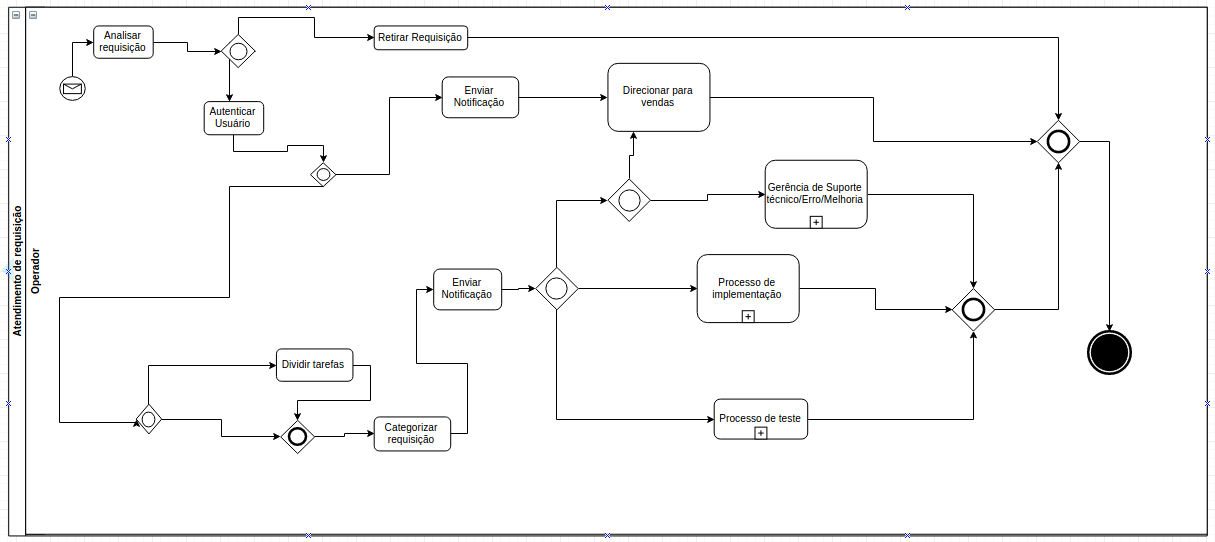
\includegraphics[width=15cm]{to_be/01_atendimento_de_requisicao.png}
\label{figura:atendimento_requisicao_to_be}
\end{figure}

Como primeira ação foi necessário achar os indicadores chave de performace,
onde foi possivel mapear o relacionamento desses indicadores chave com os fatores
\cite{cartlidge2007introductory} criticos de sucesso

\subsubsection{Atendimento técnico}
\begin{figure}[!h]
\caption{Atendimento técnico}
\centering % para centralizarmos a figura
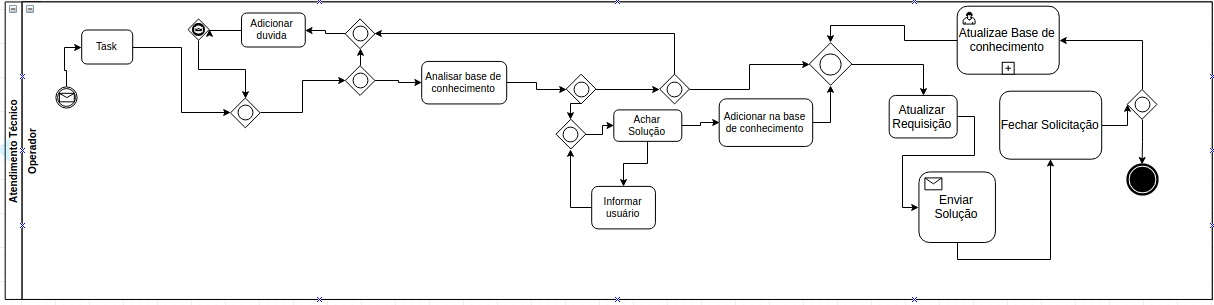
\includegraphics[width=15cm]{to_be/02_atendimento_tecnico.png}
\label{figura:suporte_tecnico_to_be}
\end{figure}



\subsubsection{Atendimento para erro no sistema}

\begin{figure}[!h]
\caption{Atendimento para erro no sistema}
\centering % para centralizarmos a figura
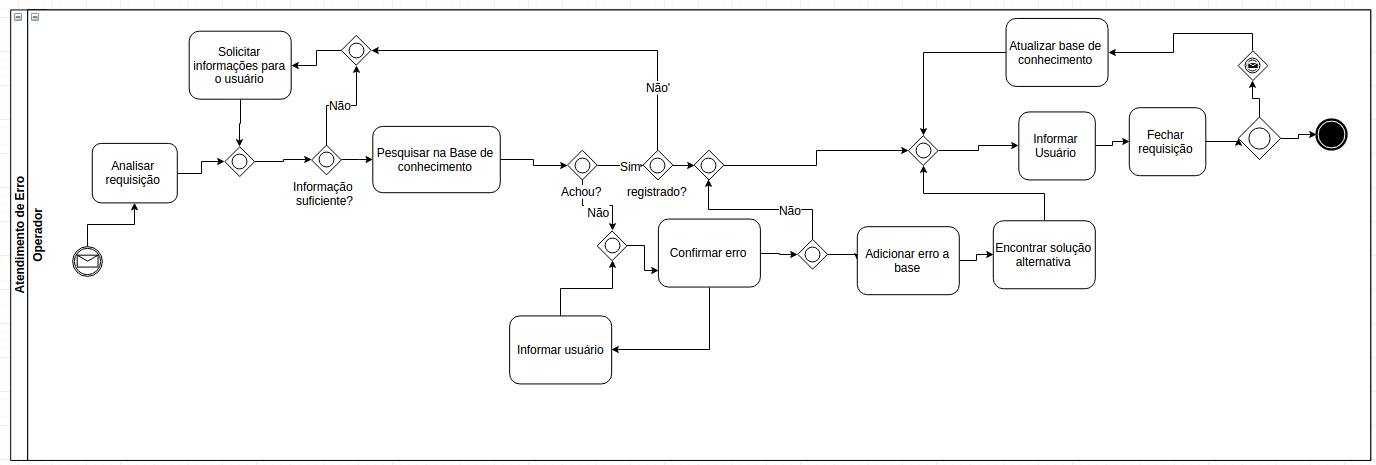
\includegraphics[width=15cm]{to_be/03_atendimento_de_erro.png}
\label{figura:atendimento_de_erro_to_be}
\end{figure}
